\chapter{Projektplanlægning}

Indledningsvis kom vi ind på, at vi har brugt Asana til projektstyring.
På Asana har vi delt projektet op i forskellige \textit{tasks} og uddelegeret opgaverne lige og ladet alle bidrage til alle opgaverne.
Det ses i \ref{fig:Asana}, at programmet er opddelt i tre spalter; \textit{tasks}, \textit{in progress} og \textit{done}, som dynamisk ændrer sig gennem projektforløbet.

\begin{figure}[h]
    \begin{center}
        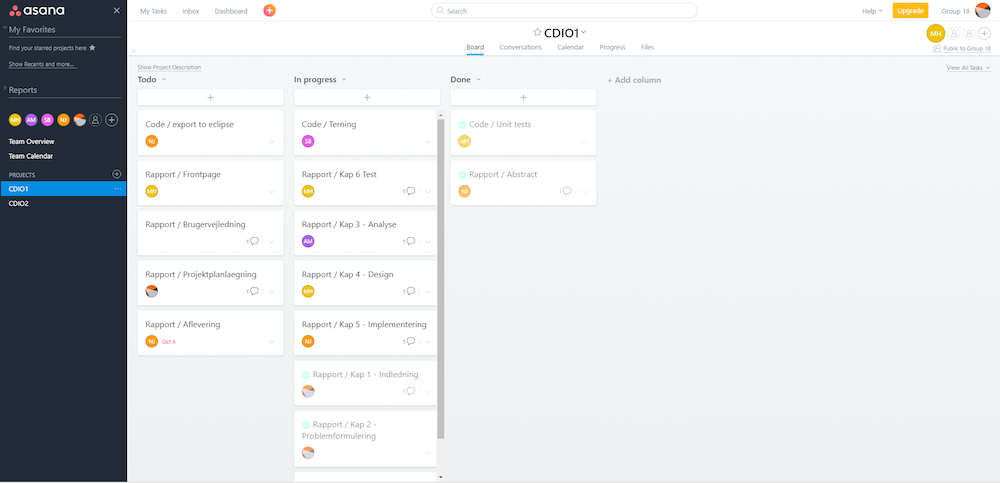
\includegraphics[width=15cm]{graphics/Asana}
        \caption{Screendump af Asana}
        \label{fig:Asana}
    \end{center}
\end{figure}

\noindent
Asana understøtter UP, idet man kan oprette x-antal tasks som eksempelvis 'inception' og 'elaboration' og derefter lave x-antal \textit{subtasks}, som kan svare til iterationer.

\pagebreak

\noindent
Diagrammet herunder er inddelt i dage indtil aflevering (10 dage).  \\ Diagrammet viser den reelle tid der er brugt ved projektet.
%
%   GANTT DIAGRAM 1
%
\begin{center}
    \begin{ganttchart}[
        canvas/.append style={fill=none, draw=black!10, line width=2pt},
        hgrid style/.style={draw=black!10, line width=2pt},
        vgrid={*1{draw=black!10, line width=1pt}},
        title/.style={draw=none, fill=none},
        title label font=\bfseries\footnotesize,
        title label node/.append style={below=.3pt},
        include title in canvas=false,
        bar label font=\mdseries\small\color{black!70},
        bar label node/.append style={left=2pt},
        bar/.append style={draw=none, fill=black!50},
        bar incomplete/.append style={fill=barblue},
        bar progress label font=\mdseries\footnotesize\color{black!70},
        group incomplete/.append style={fill=groupblue},
        group left shift=0,
        group right shift=0,
        group height=.3pt,
        group peaks tip position=0,
        group label node/.append style={left=.3cm},
        group progress label font=\bfseries\small,
        link/.style={-latex, line width=1.5pt, linkred},
        link label font=\scriptsize\bfseries,
      ]{1}{20}

      %
      % Ganttgroup laver den store fyldige overgruppe
      % Ganttbar laver de små linjer
      % De tal der er ude i siden skriver man fra og til i.
      %

    \gantttitlelist{1,...,10}{2}                                    \\

        \ganttgroup {\underline{Analyse/planlægning -}} {1}{6}      \\
        \ganttbar   {Krav/opgaveanalyse}                {1}{4}      \\
        \ganttbar   {Projektopsætning/plan}             {1}{1}      \\
        \ganttbar   {Tildeling af opgaver}              {2}{2}      \\

        \ganttgroup {\underline{Rapport -}}             {3}{20}     \\
        \ganttbar   {Analyse}                           {3}{7}      \\
        \ganttbar   {Design}                            {8}{10}     \\
        \ganttbar   {Test og implementering}            {6}{11}     \\
        \ganttbar   {Projektplanlægning}                {16}{18}    \\
        \ganttbar   {Konklusion}                        {18}{19}    \\

        \ganttgroup {\underline{Programmering -}}       {4}{13}     \\
        \ganttbar   {Test og forbedring 1}              {4}{8}      \\
        \ganttbar   {Test og forbedring 2}              {9}{13}     \\
    \end{ganttchart}
\end{center}

\pagebreak

\noindent
Diagrammet herunder er inddelt i dage indtil aflevering (10 dage).  \\ Diagrammet viser den reelle tid der er brugt ved projektet.
    
%
%   GANTT DIAGRAM 2
%
\begin{center}
    \begin{ganttchart}[
        canvas/.append style={fill=none, draw=black!10, line width=2pt},
        hgrid style/.style={draw=black!10, line width=2pt},
        vgrid={*1{draw=black!10, line width=1pt}},
        title/.style={draw=none, fill=none},
        title label font=\bfseries\footnotesize,
        title label node/.append style={below=.3pt},
        include title in canvas=false,
        bar label font=\mdseries\small\color{black!70},
        bar label node/.append style={left=2pt},
        bar/.append style={draw=none, fill=black!50},
        bar incomplete/.append style={fill=barblue},
        bar progress label font=\mdseries\footnotesize\color{black!70},
        group incomplete/.append style={fill=groupblue},
        group left shift=0,
        group right shift=0,
        group height=.3pt,
        group peaks tip position=0,
        group label node/.append style={left=.3cm},
        group progress label font=\bfseries\small,
        link/.style={-latex, line width=1.5pt, linkred},
        link label font=\scriptsize\bfseries,
      ]{1}{20}

        %
        % Ganttgroup laver den store fyldige overgruppe
        % Ganttbar laver de små linjer
        % De tal der er ude i siden skriver man fra og til i.
        %

    \gantttitlelist{1,...,10}{2}                                    \\

        \ganttgroup {\underline{Analyse/planlægning -}} {11}{16}      \\
        \ganttbar   {Krav/opgaveanalyse}                {11}{14}      \\
        \ganttbar   {Projektopsætning/plan}             {15}{16}      \\
        \ganttbar   {Tildeling af opgaver}              {14}{14}      \\

        \ganttgroup {\underline{Rapport -}}             {12}{20}      \\
        \ganttbar   {Analyse}                           {13}{13}      \\
        \ganttbar   {Design}                            {14}{14}     \\
        \ganttbar   {Test og implementering}            {15}{15}     \\
        \ganttbar   {Projektplanlægning}                {16}{16}    \\
        \ganttbar   {Konklusion}                        {17}{17}    \\

        \ganttgroup {\underline{Programmering -}}       {12}{20}     \\
        \ganttbar   {Test og forbedring 1}              {13}{16}      \\
        \ganttbar   {Test og forbedring 2}              {17}{20}     \\
    \end{ganttchart}
\end{center}